\chapter{Diseño}
\label{chap:diseño}

Para abordar el diseño de la aplicación a lo largo de este capítulo, se detallará la arquitectura software elegida para el sistema
y se mostrarán los prototipos de la interfaz de usuario.

\section{Arquitectura}
\label{sec:diseño_arquitectura}

Teniendo en cuenta los requisitos definidos en las Secciones \ref{sec:analisis_requisitos_funcionales} y \ref{sec:analisis_requisitos_no_funcionales},
así como también las limitaciones temporales del proyecto, se ha optado por una arquitectura cliente-servidor. Esta aquitectura se ha elegido
por la facilidad en su implementación y por su capacidad de intercomunicación con otros sistemas, especialmente con clientes web. Como
se aprecia en la Figura \ref{fig:arquitectura_contenedor}, el servidor cuenta con un controlador REST capaz de redirigir las peticiones al servicio
corresepondiente. En este sentido, a pesar de solo contar con un único servicio (\textit{Servicio de perfilado}) en la versión actual,
la arquitectura cliente-servidor permite añadir nuevos servicios, junto a nuevas funcionalidades, de forma sencilla y sin poner en riesgo al resto del sistema.
Dicho servicio será el que se comunique con la base da datos para garantizar la persistencia de los datos del perfilado y permitir así
una posterior consulta.

\bigskip
Por otro lado, para que el código estuviese bien organizado, se decidió utilizar el patrón de diseño DDD (del inglés \textit{Domain-Driven Design}) \cite{ddd}, el cual
permite separar el código en tres capas: la capa de aplicación, la capa de dominio y la capa de infraestructura. La capa de aplicación es la encargada de gestionar
la entrada y salida de la aplicación que, en nuestro caso, es el controlador que maneja los \textit{endpoints} REST; la capa de dominio es la que contiene la lógica
de negocio y las entidades; y la capa de infraestructura es la responsable de administrar las interacciones internas de la aplicación que, en nuestro
caso, se encarga de la comunicación con la base de datos.

\begin{figure}[H]
	\centering
	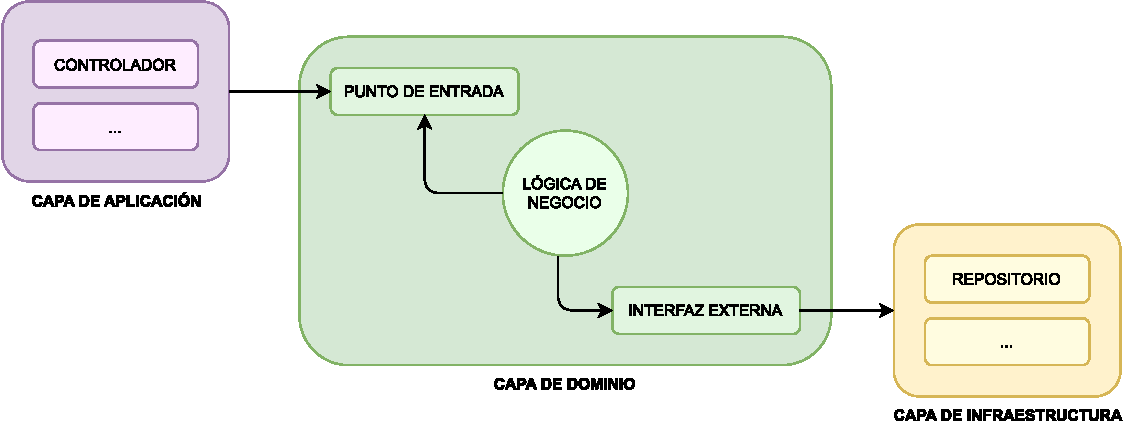
\includegraphics[width=0.9\textwidth]{diagramas/ddd.pdf}
	\caption{Diagrama de capas del patrón de diseño DDD. Adaptado de Ł, Ryś \cite{dddblog}}
	\label{fig:ddd}
\end{figure}

\bigskip
A mayores, el propio \textit{frontend} web tendrá también una arquitecture basada en cliente-servidor, en la que el servidor será el encargado
de ofrecer al cliente los archivos estáticos necesarios para mostrar la interfaz (HTML, CSS, JavaScript, fuentes, imágenes...). El hecho
de elegir una interfaz web gira en torno al requisito no funcional de portabilidad definido en la Sección \ref{sec:analisis_requisitos_no_funcionales},
puesto que de esta forma, la aplicación podría ser utilizada por cualquier dispositivo con un navegador web, evitando
desarrollar aplicaciones nativas para cada sistema operativo.

\bigskip
\begin{figure}[H]
	\centering
	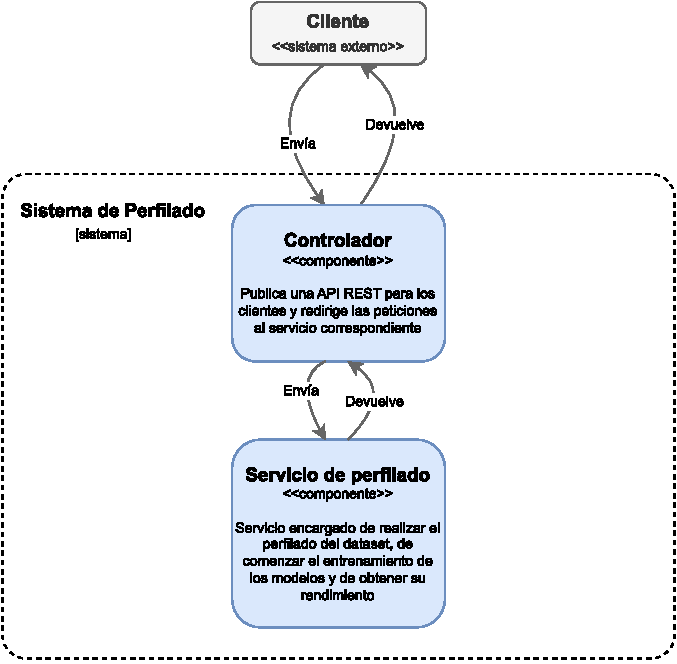
\includegraphics[width=0.7\textwidth]{diagramas/arquitectura_contenedor.pdf}
	\caption{Diagrama C4 de Contenedor de la arquitectura del sistema.}
	\label{fig:arquitectura_contenedor}
\end{figure}

\section{Prototipado}
\label{sec:diseño_prototipado}

Como se mencionó anteriormente, para el diseño de los prototipos de pantallas, también conocidos como \textit{wireframes}, se utilizó
la herramienta Draw.io \cite{drawio} debido a su sencillez y rapidez en la elaboración con respecto a otros programas más avanzados
como pueden ser Adobe XD \cite{adobexd} o Figma \cite{figma}.

\bigskip
La filosofía de diseño de la interfaz se centró en el minimalismo y la usabilidad, como se indica en la Sección \ref{sec:analisis_requisitos_no_funcionales}
, por lo que todo estará caracterizado por no contener excesivos elementos y por ser fácilmente comprensible para el usuario. 

\bigskip
La pantalla de inicio, como se ve en la Figura \ref{fig:prototipo_inicio}, está compuesta simplemente por un título, 
un subtítulo y un campo que permitirá al usuario subir un \textit{dataset}, tanto mediante un elemento \textit{drag and drop} como
mediante un botón que abrirá el explorador de archivos del sistema operativo.

\bigskip
\begin{figure}[H]
	\centering
	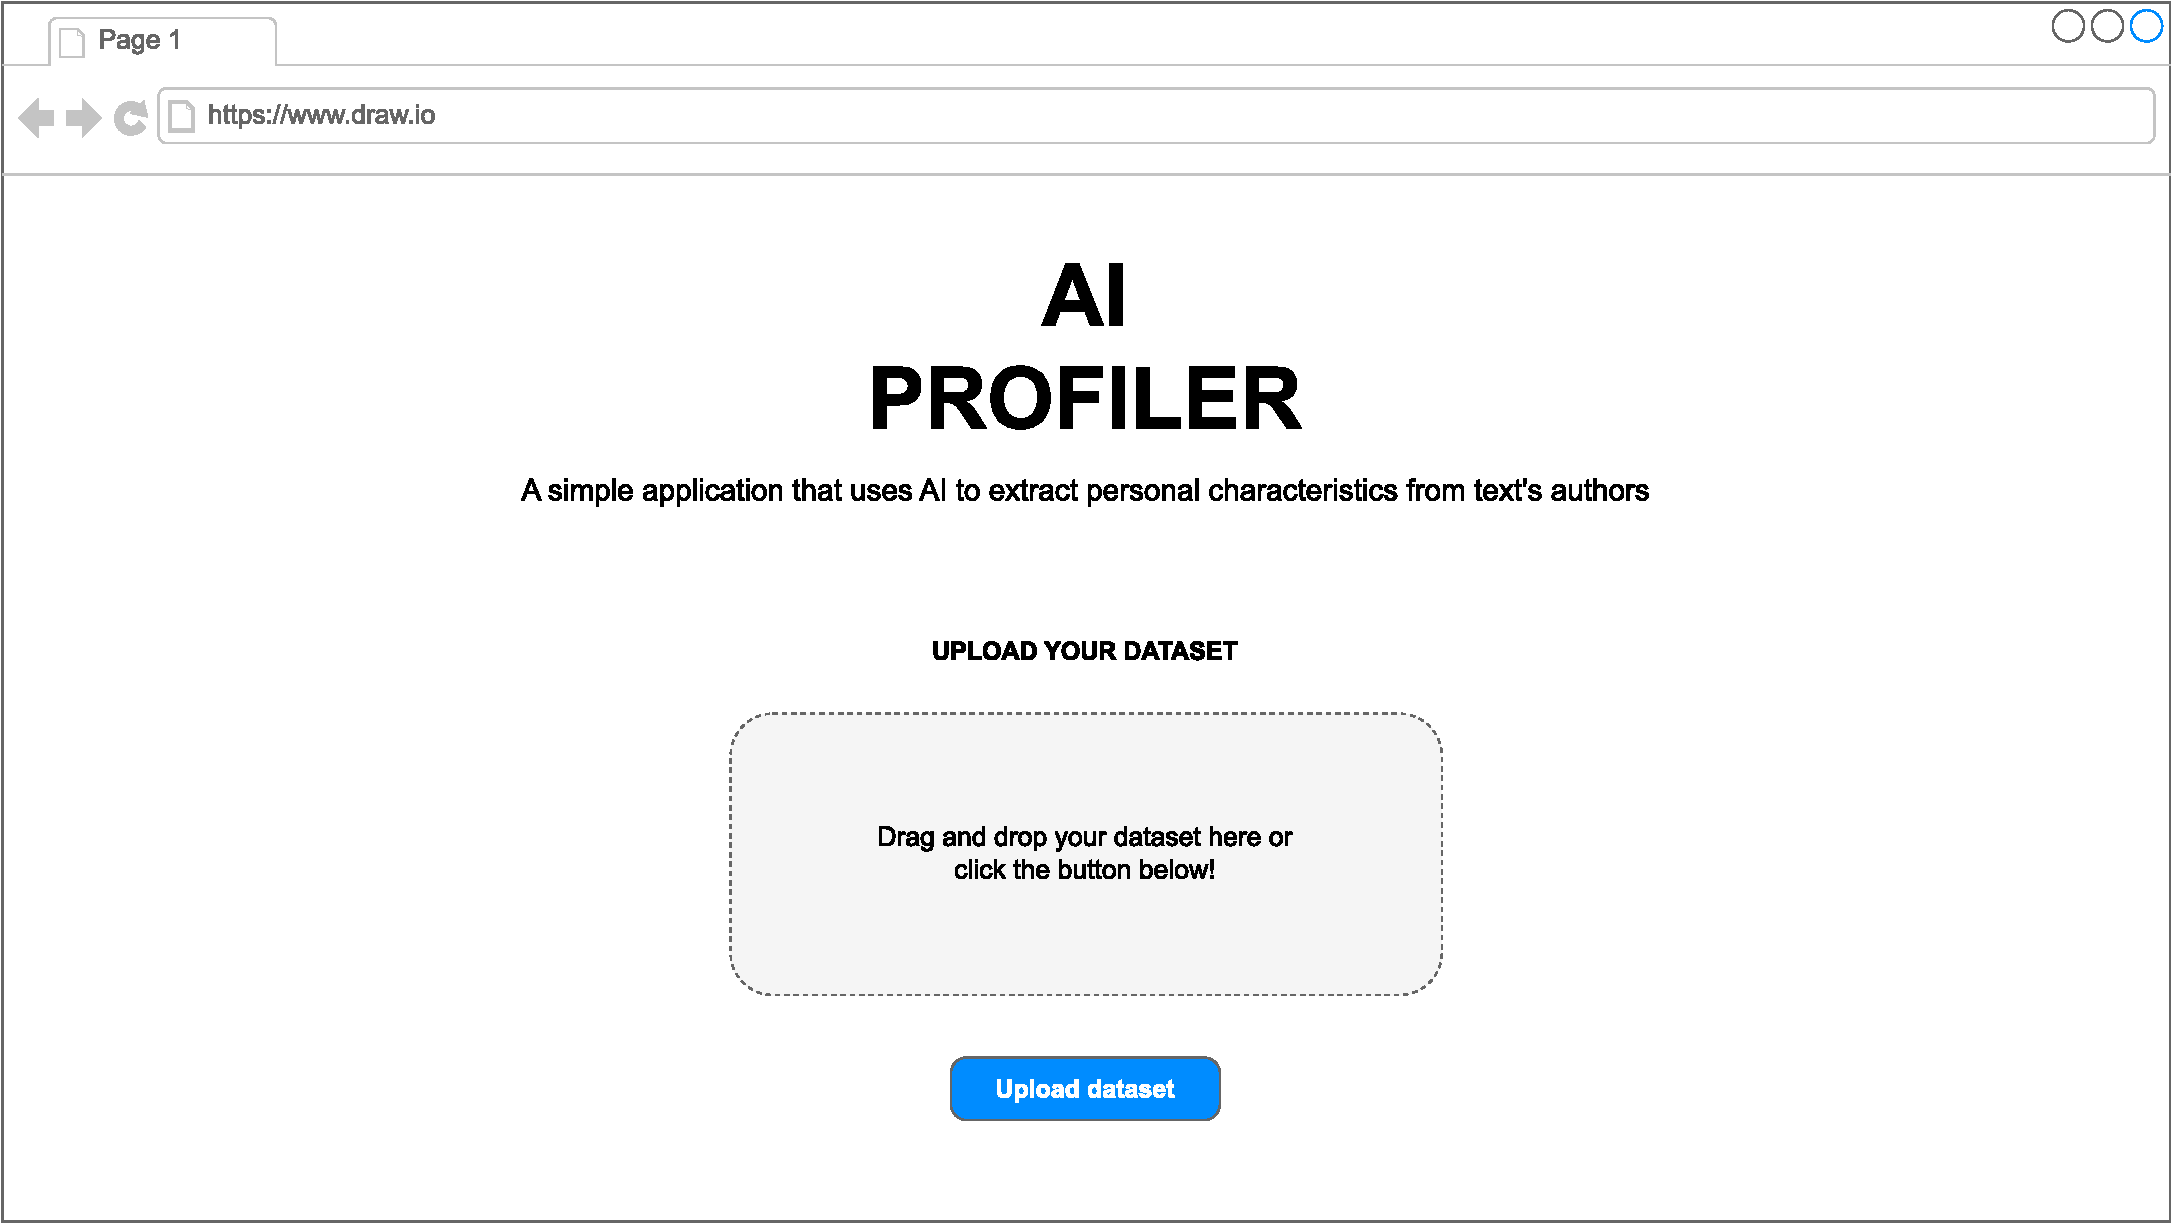
\includegraphics[width=\textwidth]{diagramas/landing.pdf}
	\caption{Prototipo de la pantalla de inicio}
	\label{fig:prototipo_inicio}
\end{figure}

\bigskip
Una vez el usuario haya subido el \textit{dataset}, el campo de subida se sustituirá por la lista de los
algoritmos de perfilado disponibles, como se puede ver en la Figura \ref{fig:prototipo_algoritmo_perfilado}. De cada algoritmo se mostrará, en una tarjeta, las características que es capaz de extraer
del perfilado junto con su título. Además, ya que uno de los requisitos era el de mostrar información del funcionamiento
y del rendimiento de los algoritmos, se decidió crear un \textit{tooltip} que se mostrase cada vez que el usuario pasase el ratón
por encima de cada tarjeta. Finalmente, si el usuario desease cambiar el \textit{dataset} seleccionado, se permitirá retroceder mediante
la flecha situada junto al título del paso actual.

\bigskip
\begin{figure}[H]
	\centering
	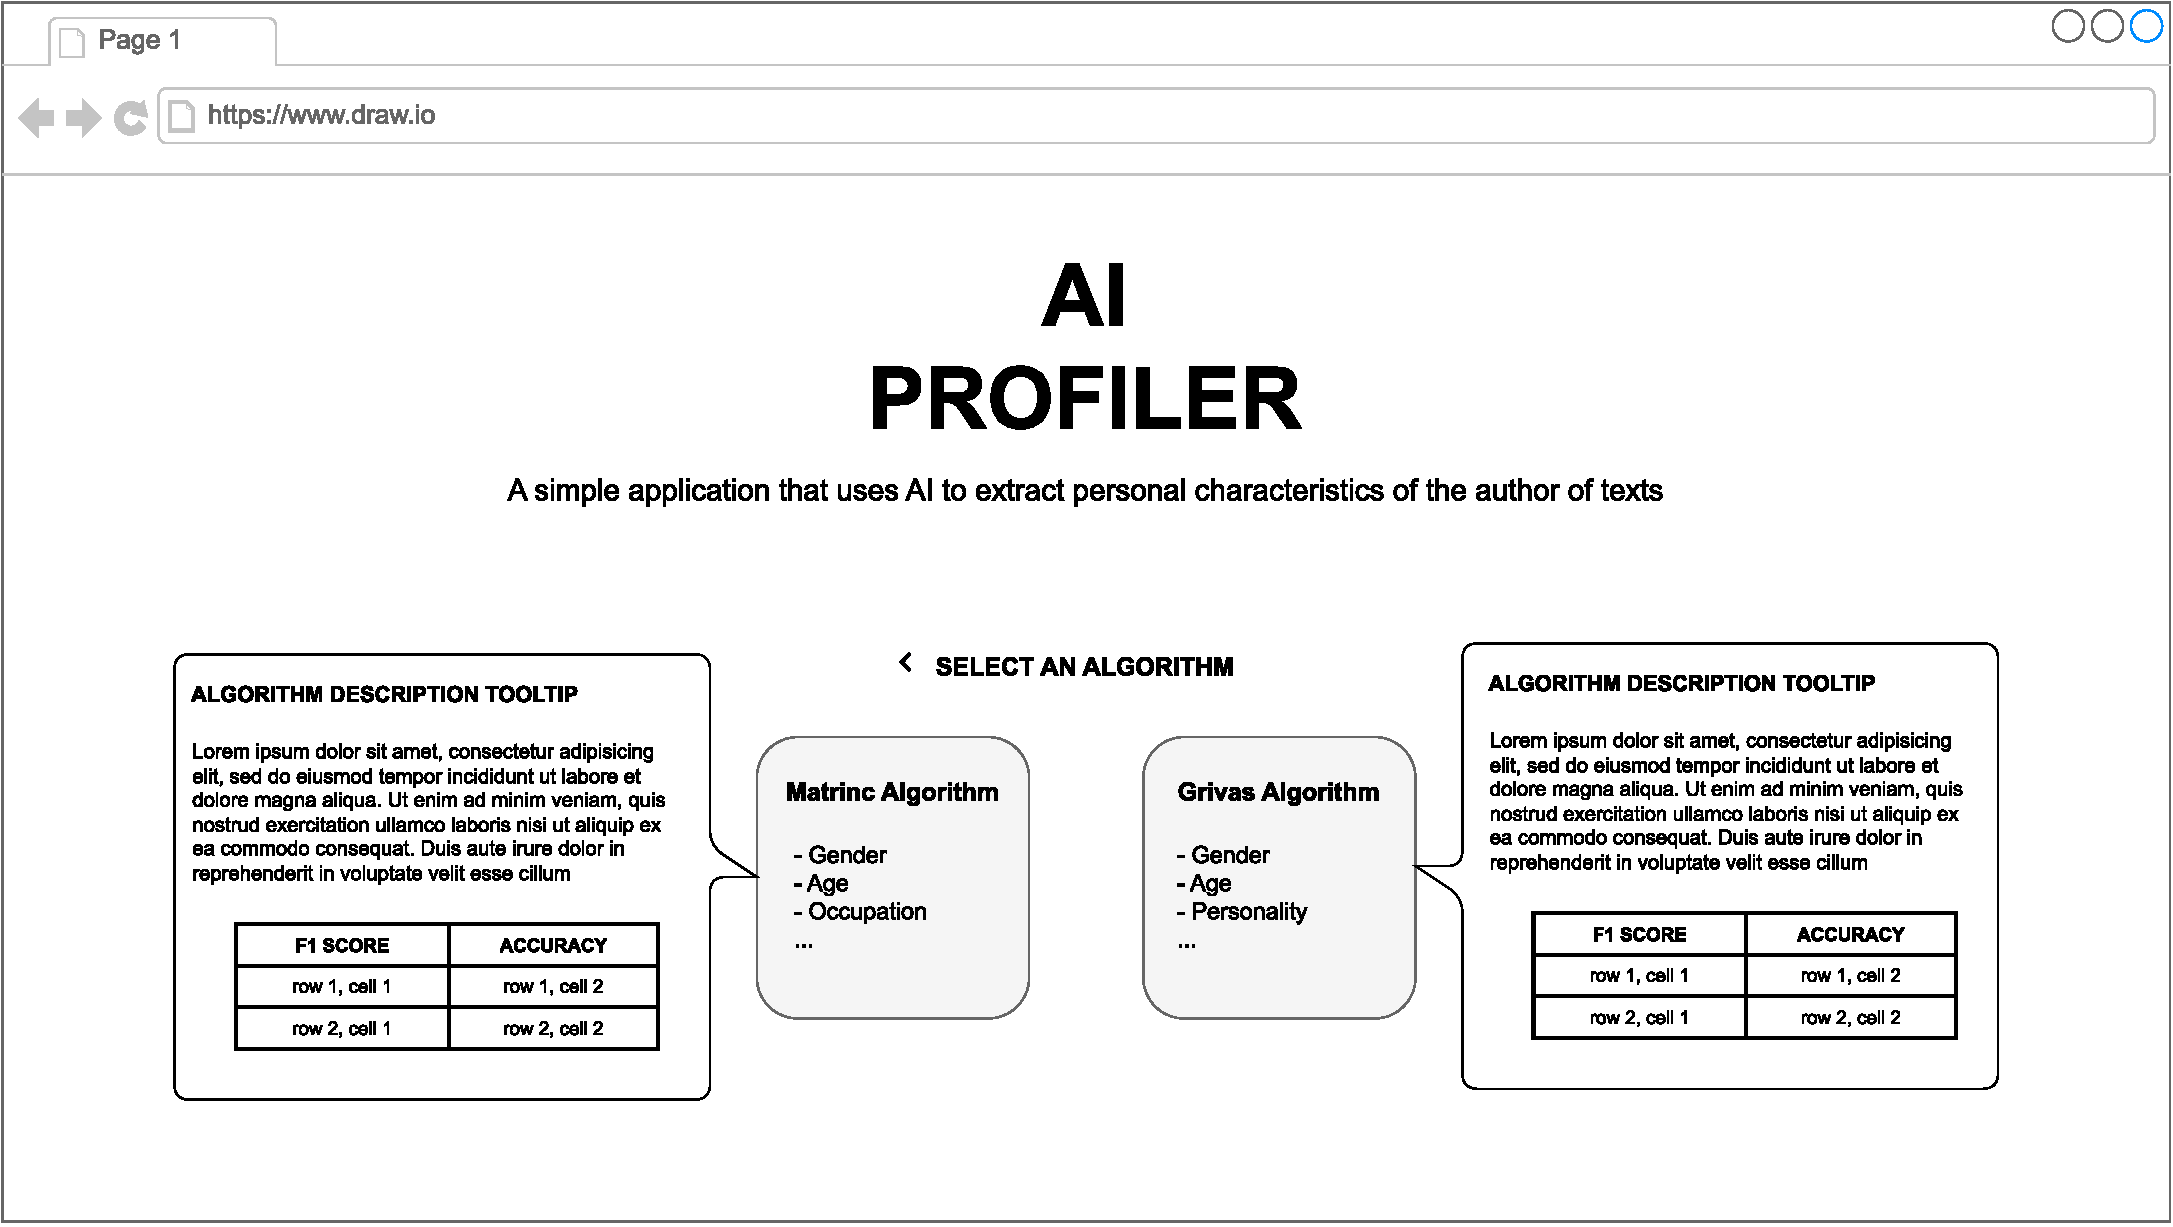
\includegraphics[width=\textwidth]{diagramas/landing-algorithm.pdf}
	\caption{Prototipo de la selección del algoritmo de perfilado}
	\label{fig:prototipo_algoritmo_perfilado}
\end{figure}

\bigskip
Ya con el \textit{dataset} y el algoritmo seleccionados, se presentará al usuario un resumen del perfilado, donde se mostrará
el nombre del fichero subido, la tarjeta del algoritmo seleccionado y un botón que permitirá al usuario comenzar con el proceso de perfialdo.
Además, como se aprecia en la Figura \ref{fig:prototipo_resumen_perfilado}, una vez comienza el perfilado, se mostrará una barra de progreso
o un \textit{spinner} que le indicará al usuario que el proceso está en marcha. De la misma forma que en el paso anterior, si el usuario
decide cambiar de algoritmo, puede retroceder haciendo uso de la flecha situada junto al título del paso actual.

\bigskip
\begin{figure}[H]
	\centering
	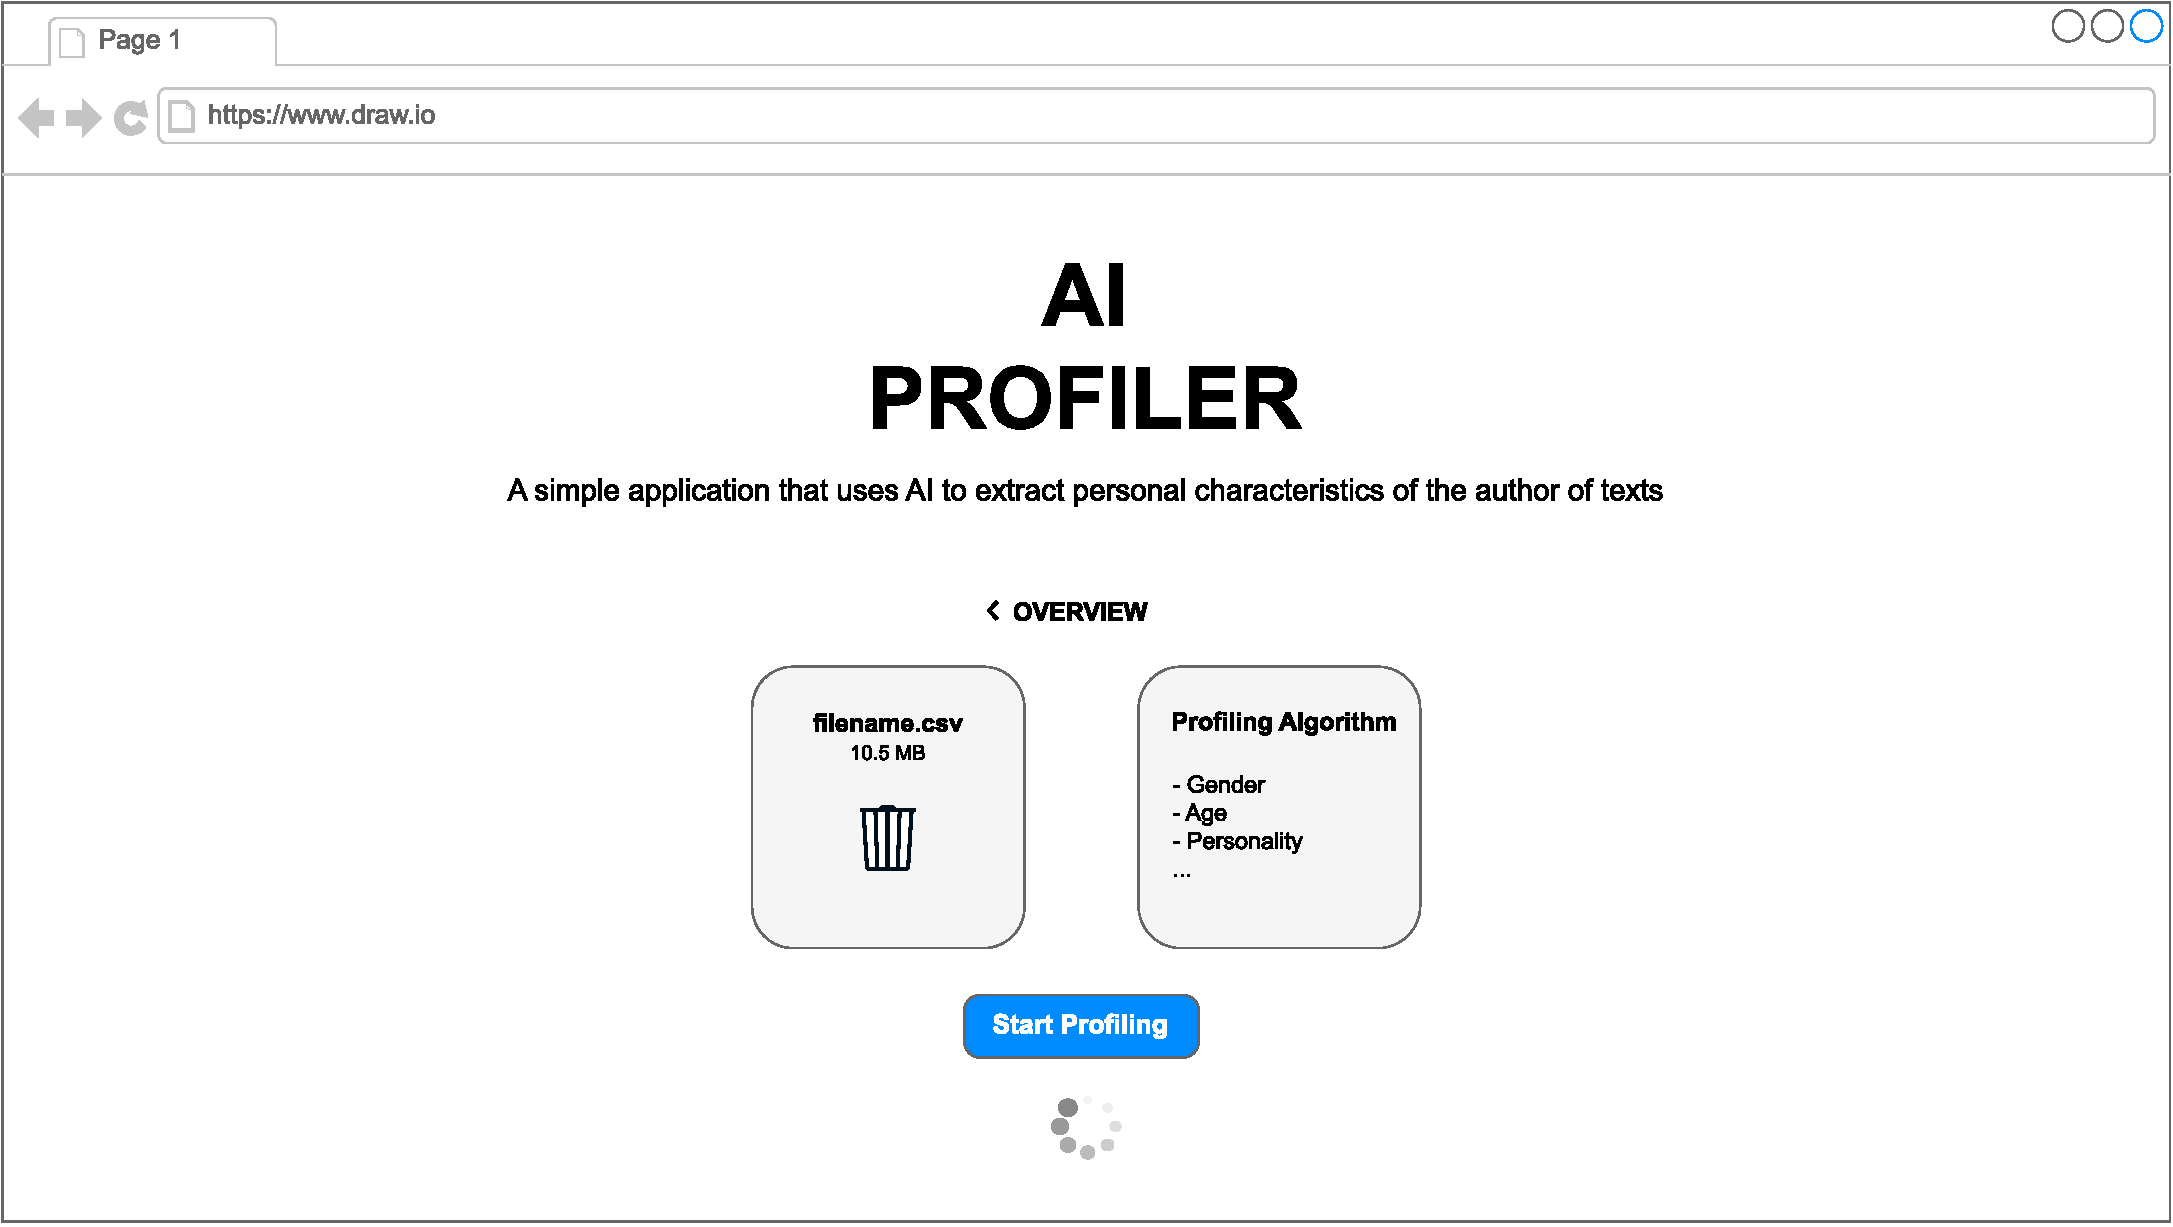
\includegraphics[width=\textwidth]{diagramas/landing-overview.pdf}
	\caption{Prototipo del resumen del perfilado}
	\label{fig:prototipo_resumen_perfilado}
\end{figure}

\bigskip
Con respecto a la pantalla de ejemplos de \textit{datasets}, como se puede ver en la Figura \ref{fig:prototipo_ejemplos_dataset},
se mostrará un pequeño ejemplo de 10-15 líneas aproximadamente. Asimismo, se le dará la opción al usuario de seleccionar el 
formato de \textit{dataset}, ya sea NDJSON o CSV, dado que son los que soportará el \textit{backend}.

\bigskip
\begin{figure}[H]
	\centering
	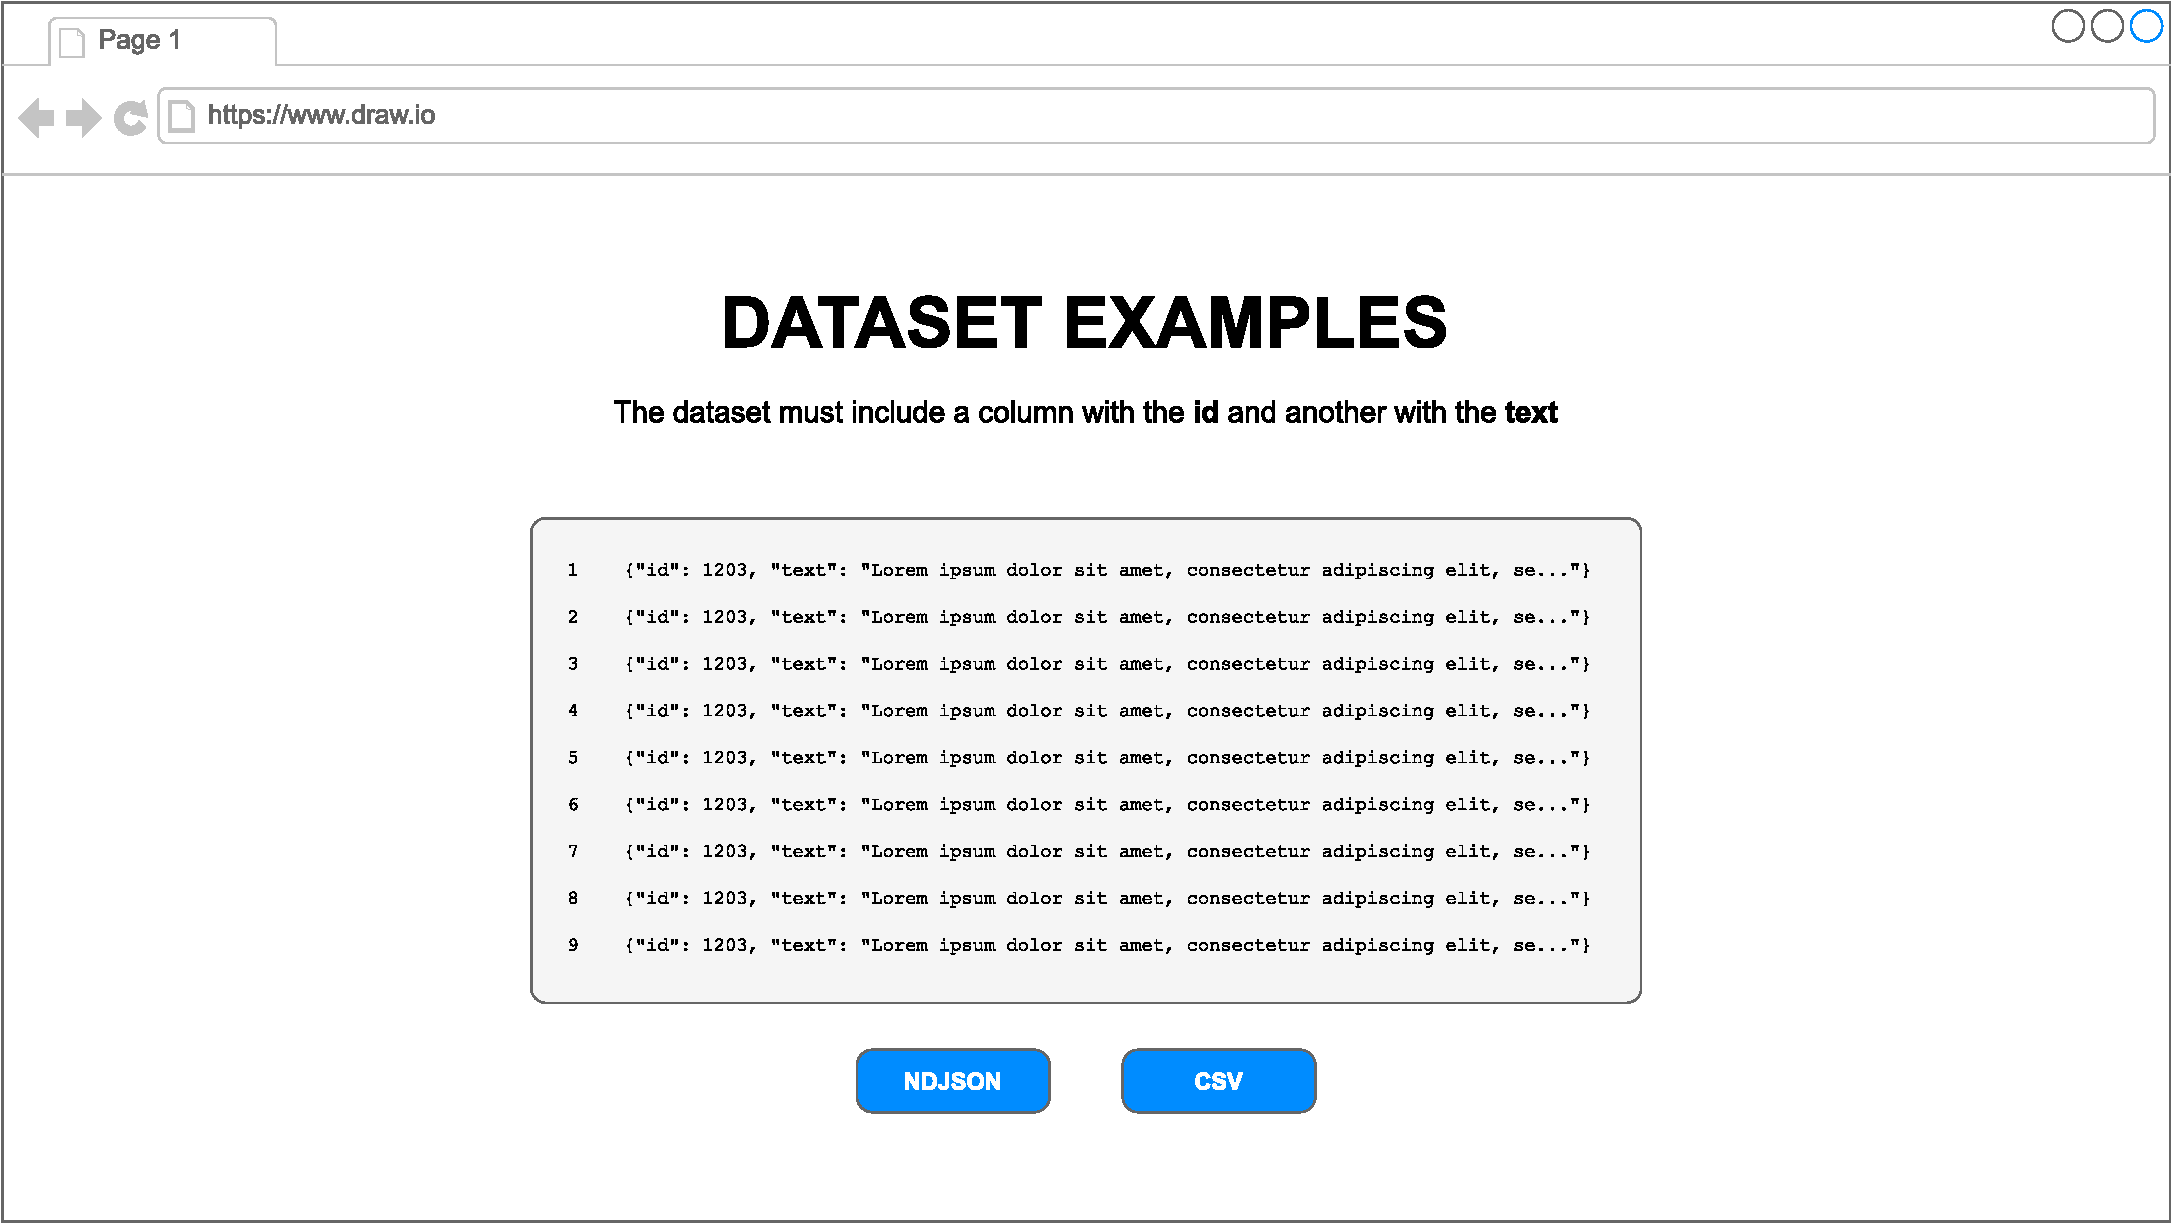
\includegraphics[width=\textwidth]{diagramas/dataset-examples.pdf}
	\caption{Prototipo de la pantalla de ejemplos de dataset}
	\label{fig:prototipo_ejemplos_dataset}
\end{figure}

\bigskip
Cuando el perfilado haya finalizado, se mostrará al usuario un \textit{dashboard} con los resultados obtenidos,
como se puede ver en las Figuras \ref{fig:prototipo_dashboard_martinc}, \ref{fig:prototipo_dashboard_grivas}. 
Este \textit{dashboard} contendrá los siguientes gráficos y elementos, los cuales variarán en función del algoritmo utilizado:

\begin{itemize}
	\item \textbf{Datos generales}: El \textit{dashboard} contiene una primera sección en la que aparece información de carácter general
		como son: el número total de personas perfiladas, el tiempo total del perfilado y el algoritmo utilizado.
	\item \textbf{Lista detallada de personas}: En esta sección, se muestra la lista de personas perfiladas de forma paginada. Además, la lista
		permitirá ser ordenada por cada uno de los diferentes campos, según se indica en la historia de usuario con identificador 
		\textit{6} de la Sección \ref{sec:analisis_requisitos_funcionales}. Para ello, el usuario deberá hacer clic en el nombre de dicho campo, teniendo
		la opción de, volviendo a clicar, cambiar el sentido de ordenación (ascendente o descendente).
	\item \textbf{Distribución de edad}: Para la distribución de edad, se ha optado por un gráfico de barras sobre otras opciones de representación
		categóricas como el gráfico circular. Esto se debe a que, teniendo cinco clases diferentes, el gráfico de barras permite una mejor visualización 
		de los datos y una comparativa más clara entre ellos, dado que es más fácil comparar longitudes que áreas o ángulos. En la parte inferior del gráfico,
		se mostrará una tarjeta con la edad mediana.
	\item \textbf{Distribución de género}: En cuanto a la distribución de género, en cambio, se ha optado por un gráfico circular, puesto que solo existen dos clases
		y se desea resaltar la proporción de cada clase con respecto al total. A mayores, se mostrarán debajo del gráfico dos tarjetas con el número de personas
		de cada género junto con su porcentaje exacto.
	\item \textbf{Distribución de fama \textit{(Martinc)}}: De forma similar a la distribución de género, solo contamos con tres clases diferentes, por lo que
		se ha elegido un gráfico circular. Resaltar que este gráfico solo se mostrará en el caso de que se haya utilizado el algoritmo de Martinc.
	\item \textbf{Distribución de ocupación \textit{(Martinc)}}: En el caso de la distribución de ocupación, debido a que existen ocho clases distintas, se ha optado
		por un gráfico de barras. Este gráfico, al igual que el anterior, solo aparecerá si se ha empleado el algoritmo de Martinc para el perfilado.
	\item \textbf{Características personales \textit{(Grivas)}}: Ya que en este caso cada característica personal tendría asociado un valor decimal entre -0.5 y 0.5,
		se ha optado por un gráfico de barras. En este sentido, cabe resaltar que para mostrar dicho gráfico, es necesario implementar una funcionalidad que permita
		seleccionar a una persona de la lista detallada para mostrar sus características personales. Además, este gráfico solo estará disponible si se hace uso del algoritmo de Grivas.
\end{itemize}

\bigskip
\begin{figure}[H]
	\centering
	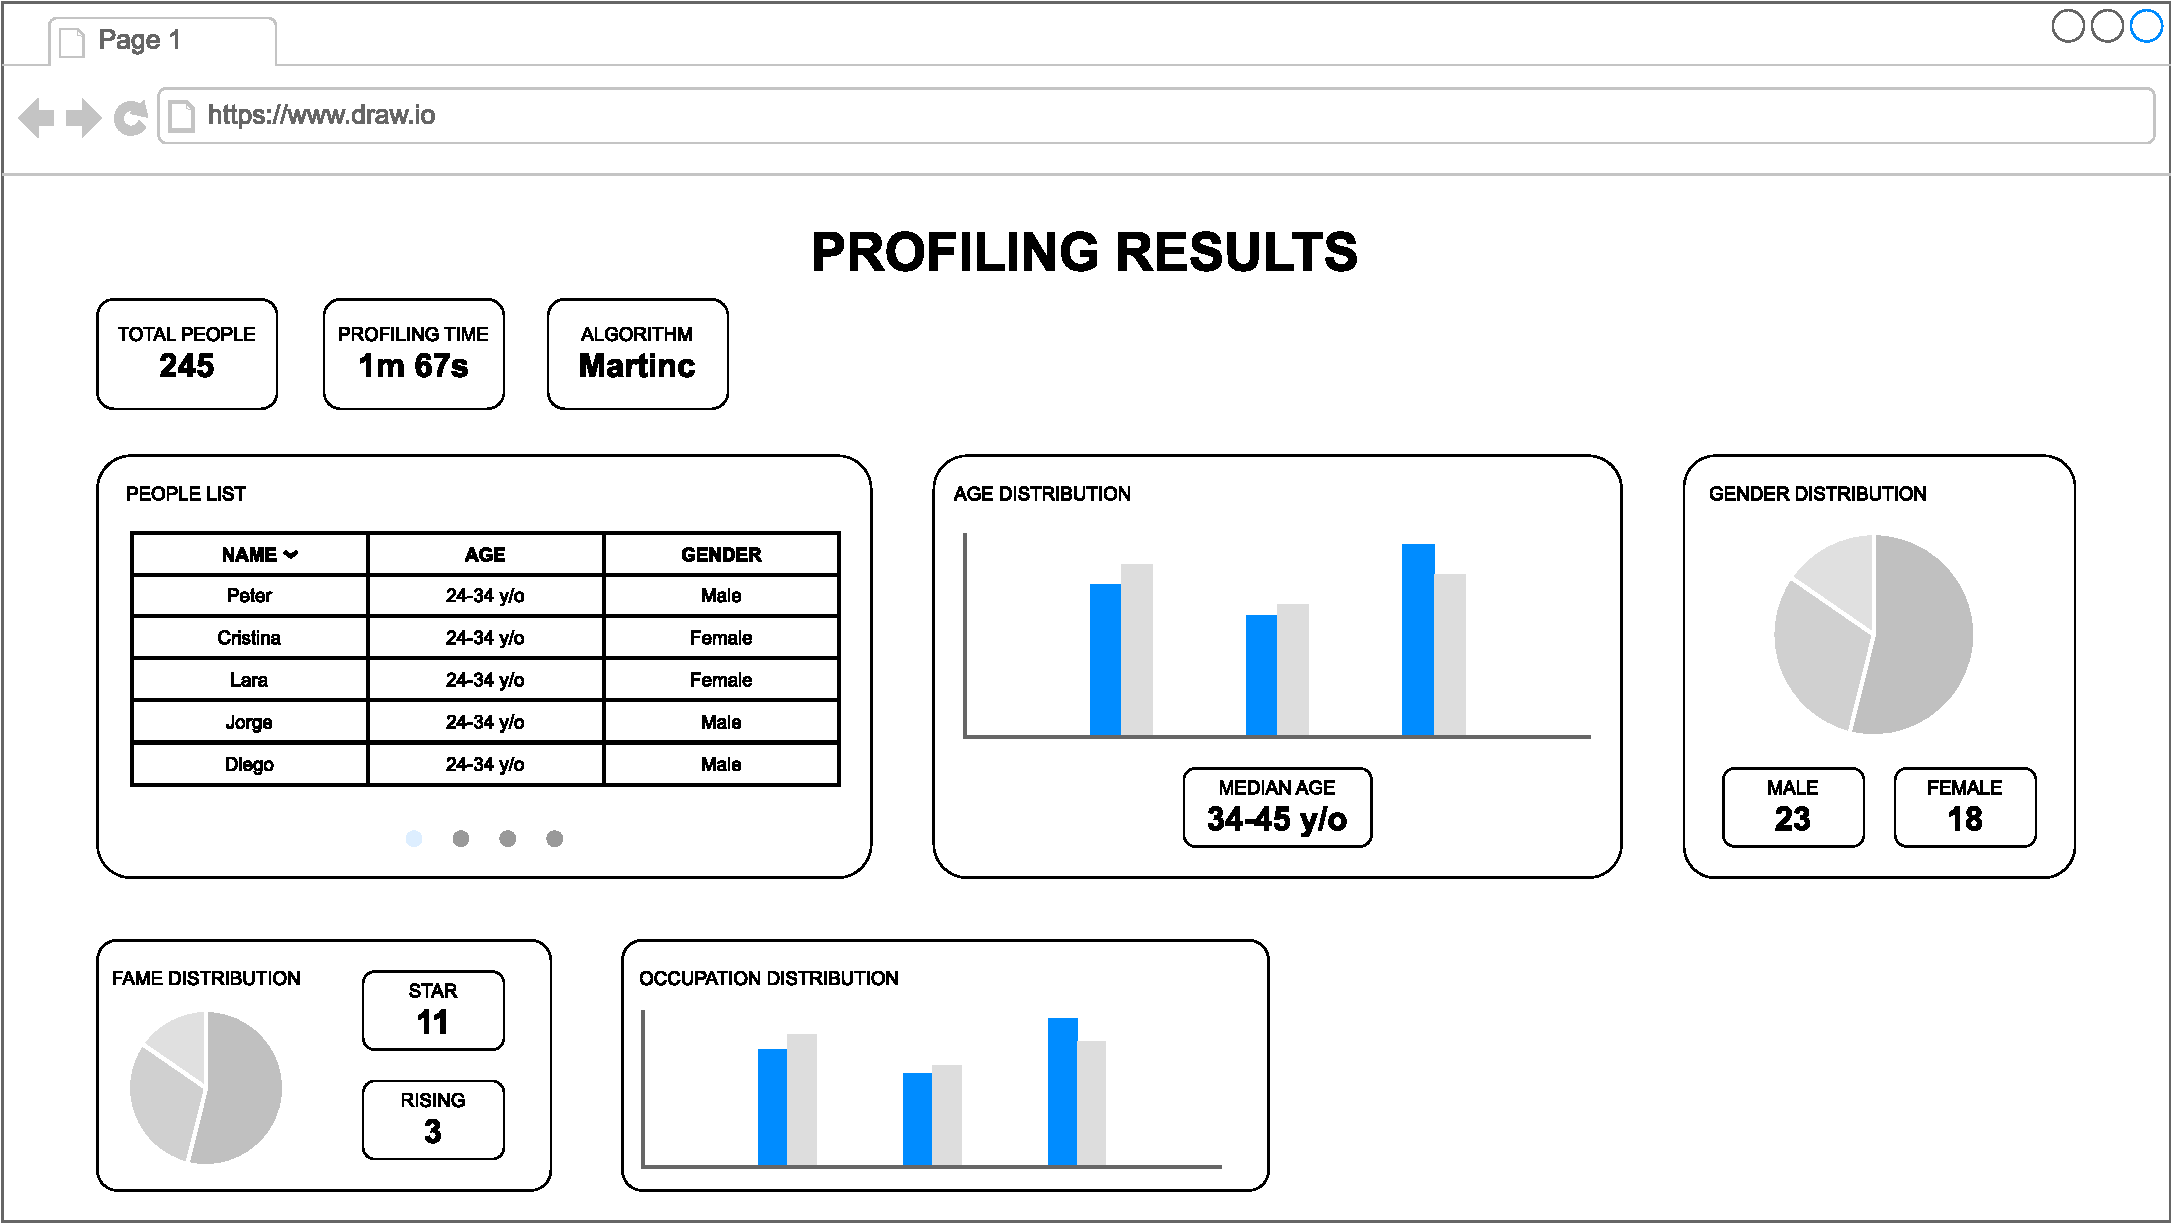
\includegraphics[width=\textwidth]{diagramas/dashboard-martinc.pdf}
	\caption{Prototipo del dashboard utilizando el algoritmo Martinc}
	\label{fig:prototipo_dashboard_martinc}
\end{figure}

\bigskip
\begin{figure}[H]
	\centering
	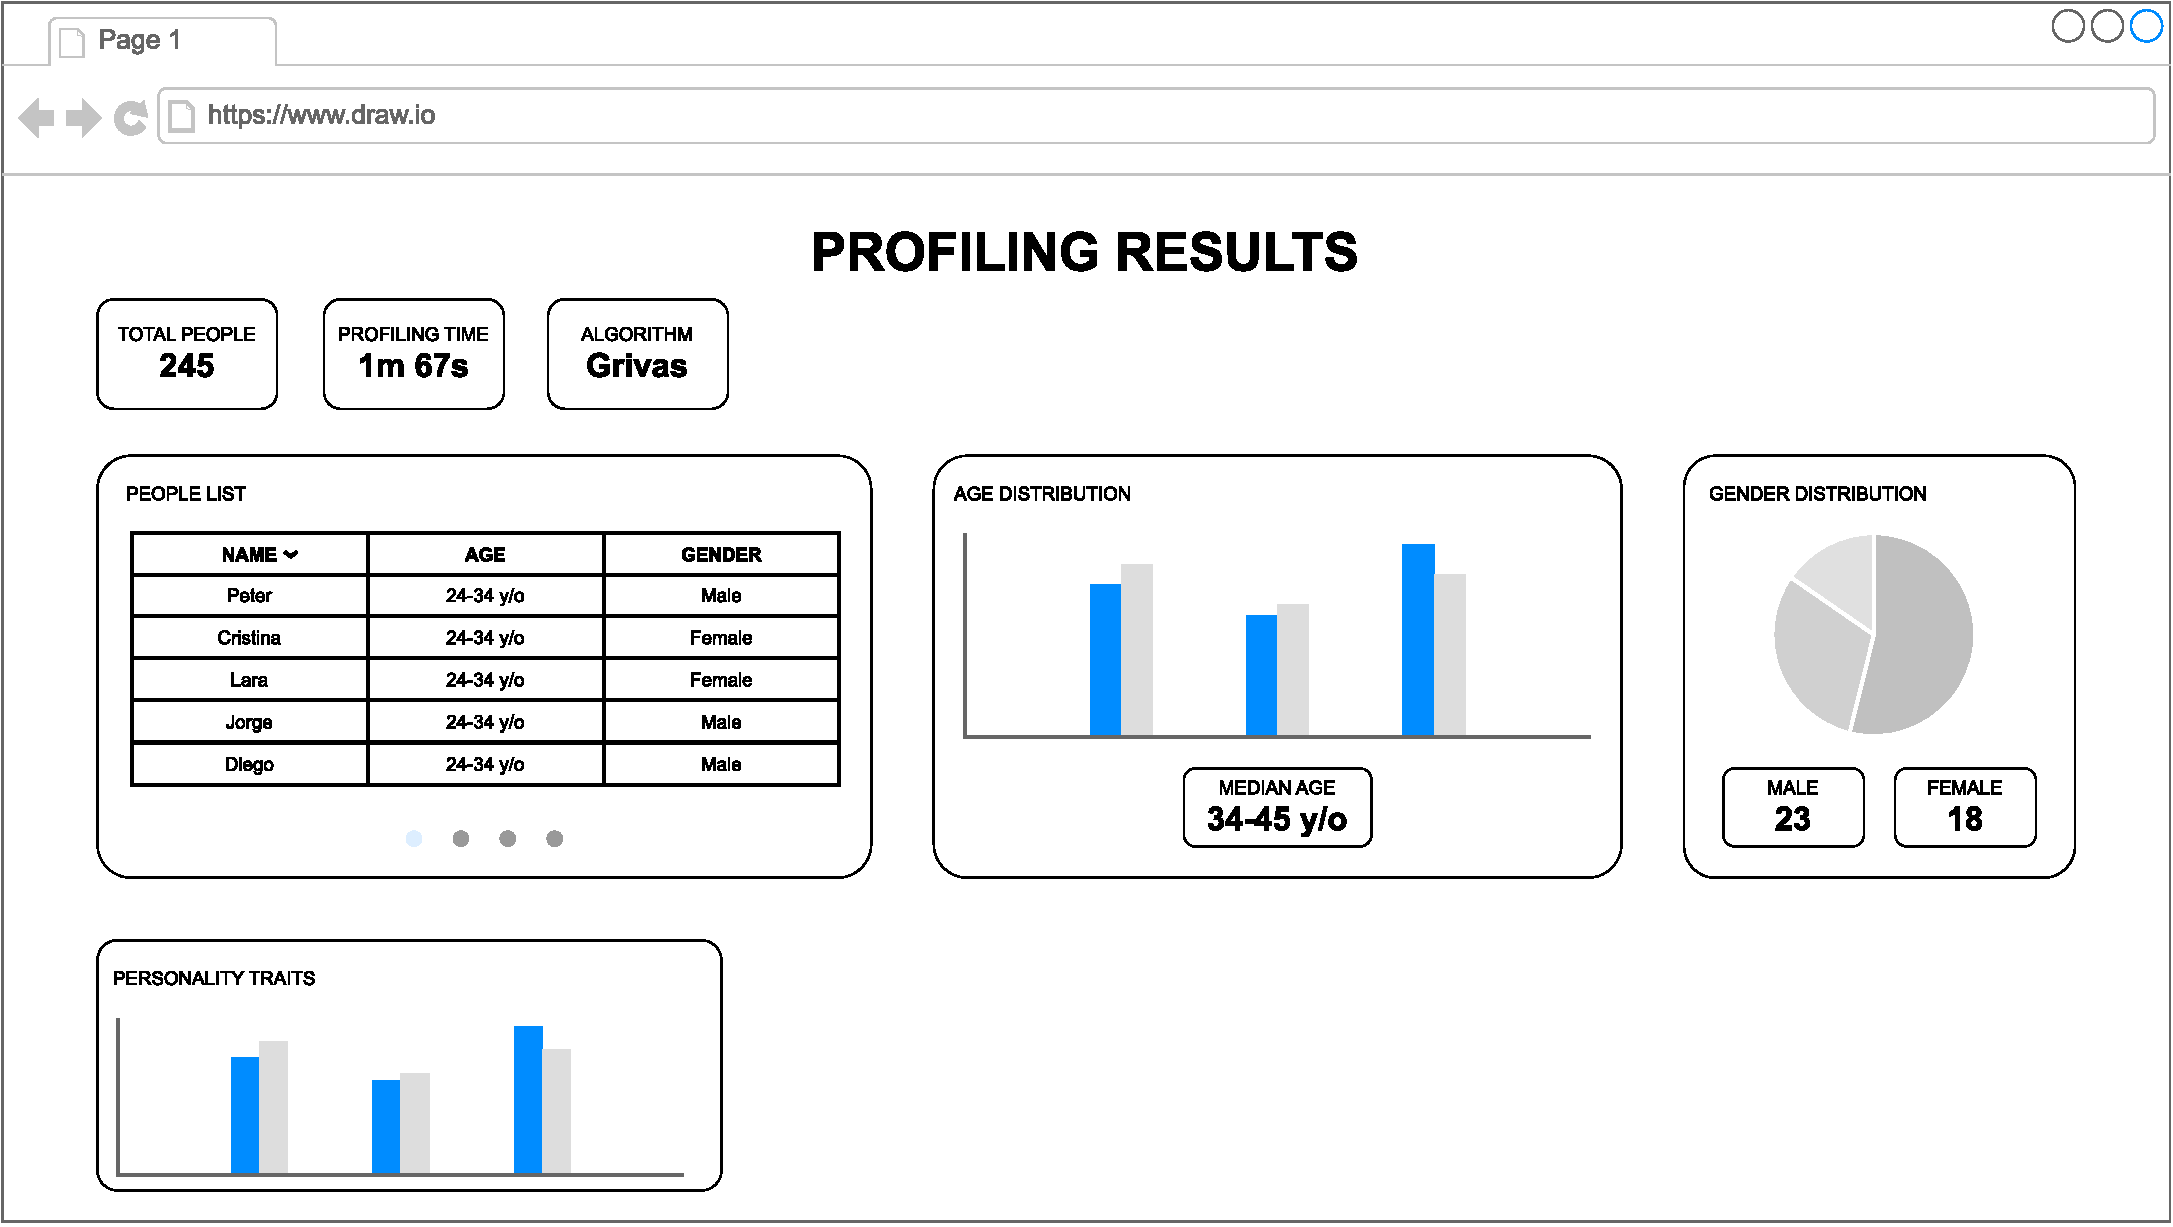
\includegraphics[width=\textwidth]{diagramas/dashboard-grivas.pdf}
	\caption{Prototipo del dashboard utilizando el algoritmo Grivas}
	\label{fig:prototipo_dashboard_grivas}
\end{figure}
